\documentclass[titlepage]{jsarticle}
\usepackage{graphicx}
\usepackage{mediabb} %bbファイルの取得用sty

\title{英文法の基礎\\ 論理的に英文を読む/書くために必要な知識のまとめ\\【Ver. 2012.3.3】
}  %%%%% タイトル
\author{文責:木村修平\\Email: kimuras@fc.ritsumei.ac.jp / Twitter: @syuhei}     %%%%%
%\date{2009年7月13日}                         %%%%% 提出日
\markright{\footnotesize \sf 英文法の基礎}

\begin{document}
\maketitle
\tableofcontents

\newpage


\setcounter{section}{-1}
\section{はじめに}
この教材は、英文法の知識に基づいて論理的に英文を読む/書くために必要な知識を、
出来る限りわかりやすく、かつ、コンパクトにまとめたものです。

この教材は、次のような読者を想定して作られています。
\begin{itemize}
\item 英語が苦手な高校生
\item 英語が苦手な大学生、特に受験科目で英語を勉強せずに入学した大学生
\item 英語によるコミュニケーションは問題ないけれど、文法知識に自信のない帰国子女
\item 英語の勉強をやり直したい社会人
\end{itemize}


\subsubsection*{【この教材を利用したい英語教員の方へ】}
もし英語教員の方などでこの教材をご自身の授業で使いたいという方がおられましたら、どうぞご自由にご利用ください。内容の加筆・改変はもちろん、再配布もご自由に行なっていただいて構いません。この教材は、「クリエイティブ・コモンズ 表示 - 非営利 - 継承 2.1 日本 ライセンス」の下に提供されています。この教材の電子データ(Word形式・PDF形式)の入手およびライセンスの詳細につきましては、下記URLをご覧ください。

【Mt. English Project:http://mep.papiko.com/】


\section{語と品詞}
ここでは、英文に含まれている語と品詞の関係について説明します。

英語で書かれた文を{\bf 英文}と呼びます。英文は複数の{\bf 語}(=単語)によって形作られています。たとえば次の英文は4つの語で成り立っています(図 \ref{fig1})。
 
 \begin{figure}[htbp]
  \begin{center}
   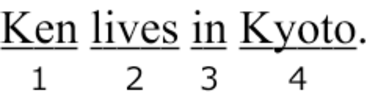
\includegraphics[width=5cm]{./figure/fig1.pdf}
   \caption{4つの語で作られた英文}
   \label{fig1}
  \end{center}
 \end{figure}
 
英文に含まれるすべての語は何らかの{\bf 品詞}に分類することができます。語と品詞の関係は、コンビニで売られている商品とその裏側に記載されているバーコードとの関係に似ています。つまり、コンビニの商品のひとつひとつにバーコードがくっついているように、英文の中の語のひとつひとつに品詞というバーコードがついているのです。

先ほどの英文に含まれる語をひっくり返して品詞=バーコードを確認してみましょう(図 \ref{fig2})。

 \begin{figure}[htbp]
  \begin{center}
   
\includegraphics[width=5cm]{./figure/fig2.pdf}
   \caption{4つの語で作られた英文}
   \label{fig2}
  \end{center}
 \end{figure}


それぞれの語の品詞を確認してみると、Kenには「人やモノを意味するバーコード」である{\bf 名詞}が、livesには「動作を表すバーコード」である{\bf 動詞}が、inには「場所や時間を表すバーコード」である{\bf 前置詞}が、そしてKyotoには{\bf 名詞}というバーコードがくっついていることがわかります。このように、英文の中の語はすべて何らかの品詞に分類できます。

論理的に英文を読む/書くためには、英文を品詞のレベルでとらえる必要があります。そのためには英文法の知識が必要です。そして、{\bf 英文法とは品詞レベルのルールの集まり}のことなのです。

では、品詞にはいくつの種類があるのでしょうか。英文を構成する主な品詞は次の13種類です。
\begin{enumerate}
\item 名詞(Noun / n.)
\item 代名詞(Pronoun / pron.)
\item 形容詞(Adjective / adj. / a.)
\item 副詞(Adverb / adv. / ad.)
\item 動詞(Verb / v.)
\item 前置詞(Preposition / prep.)
\item 接続詞(Conjunction / conj.)
\item 間投詞(Interjection / interj. / int.)
\item 助動詞(Auxiliary / aux.)
\item 冠詞(Article / art.)
\item 動名詞(Gerund / ger.)
\item 不定詞(Infinitive / infin. / inf.)
\item 分詞(Participle / part. / p.)
\end{enumerate}


品詞の名前を今すべて覚える必要はありません。ここで理解するべきは、{\bf 英文は、これら13の主要な品詞が組み合わさって出来ている}ということです。辞書で語の意味を調べるときには、{\bf 意味だけでなく品詞にも注目する習慣}をつけてください(図 \ref{fig3})。
 \begin{figure}[htbp]
  \begin{center}
   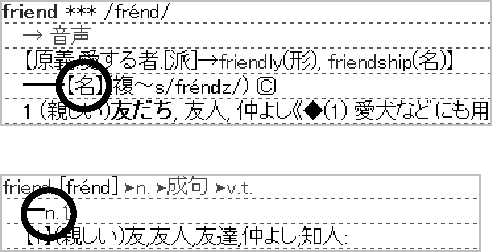
\includegraphics[width=7cm]{./figure/fig3.pdf}
   \caption{辞書で語の意味を引くときは品詞情報にも注目}
   \label{fig3}
  \end{center}
 \end{figure}
 


\end{document}
